\par This chapter presents the evaluation and results for the experiments that were discussed in Section~\ref{sec:methodology-overview}. It also addresses the research objectives mentioned in Section~\ref{subsec:research-questions-objectives}. Chapter begins with Section~\ref{sec:participant-selection}, which explains the process of selecting participants for the study. The following sections, from Section~\ref{sec:res-phase1} to Section~\ref{sec:baseline-refinement}, present detailed evaluations of each phase of the methodology. These include selecting suitable emotion recognition models, implementing the personalized multimodal fusion approach, identifying the emotional baseline, integrating emotional context into LLM responses, and refining the baseline using reinforcement learning. Each phase is evaluated using both qualitative and quantitative feedback from participants to assess how well the system addresses the defined research objectives.


\section{Participant Selection}
\label{sec:participant-selection}
For this research, we selected 10 participants using a quota sampling method combined with convenience sampling. The participants were handpicked, but not based on expert knowledge. The aim was to make sure there was a balanced representation in terms of gender, background, and age.

Out of the 10 participants, there were 6 males and 4 females. From a background point of view, 6 were from technical fields while 4 were from non-technical backgrounds. Age-wise, 2 participants were from the 15–20 age group, 5 were in the 24–26 range, and 2 were aged between 50–60.

This method helped to analyze differences in emotional expression and recognition based on these demographic factors. All participants took part with informed consent. The consent form used for this purpose is available in the Appendix (see Appendix~\ref{sec:appendix-consent}).

\section{Phase 1: Selecting Suitable Emotion Recognition Models}\label{sec:res-phase1}
In Phase 1, we mainly focused on evaluating how well different models performed when detecting emotional states using facial and vocal data. The evaluation was based on both the accuracy of emotion classification and how close the predicted intensity was to the acted intensity levels.


\subsection{Facial Expression Experiment}
This subsection discusses the results from the facial expression experiment. The emotion categorization performance of the models can be seen in Figure~\ref{fig:facial-category}, and the intensity identification results are shown in Figure~\ref{fig:facial-intensity}. In this experiment, two models were used: the HUME image expression model and CAGE.

\begin{figure}[H]
    \centering
    \includegraphics[width=1\textwidth]{img/chapter_04/facial_category_comparison}
    \caption{Emotion categorization results for facial expression experiment}
    \label{fig:facial-category}
\end{figure}

\begin{figure}[H]
    \centering
    \includegraphics[width=1\textwidth]{img/chapter_04/facial_intensity_comparison}
    \caption{Emotion intensity identification results for facial expression experiment}
    \label{fig:facial-intensity}
\end{figure}

\subsubsection*{Observation}

This section presents a structured comparison of the performance of the CAGE and HUME models in emotion category recognition and intensity measurement, based on experimental results.

\paragraph*{Emotion Category Recognition}
Both models demonstrated high accuracy in detecting certain emotions, with varying performance across categories:
\begin{itemize}
    \item \textbf{Happy}: HUME achieved 86\% accuracy, slightly outperforming CAGE at 84\%.
    \item \textbf{Sad}: HUME recorded 85\% accuracy, compared to CAGE’s 80\%, showing a modest advantage.
    \item \textbf{Angry}: Both models struggled with anger recognition. CAGE performed slightly better at 64\%, compared to HUME’s 61\%. This difficulty may stem from participants struggling to express anger naturally during the experiment.
    \item \textbf{Boredom}: HUME outperformed CAGE, with 77\% accuracy compared to CAGE’s 64\%.
    \item \textbf{Calm}: HUME achieved 74\% accuracy, while CAGE recorded 70\%, indicating a slight edge for HUME.
\end{itemize}

\paragraph*{Intensity Measurement}
HUME generally outperformed CAGE in measuring emotion intensity across all emotions:
\begin{itemize}
    \item \textbf{Happy}: HUME achieved 89\% accuracy in intensity prediction, compared to CAGE’s 81\%.
    \item \textbf{Sad}: HUME recorded 83\% accuracy, significantly outperforming CAGE’s 71\%.
    \item \textbf{Angry}: HUME achieved 58\% accuracy, compared to CAGE’s 52\%, showing a modest improvement.
    \item \textbf{Boredom}: HUME outperformed CAGE, with 81\% accuracy compared to CAGE’s 73\%.
    \item \textbf{Calm}: HUME recorded 51\% accuracy, compared to CAGE’s 47\%. Both models struggled, often confusing high calmness with low boredom.
\end{itemize}

Both models performed well in detecting happiness and sadness, with HUME showing a slight edge in category recognition for most emotions. Anger recognition remained challenging for both, likely due to unnatural expressions by participants. HUME consistently outperformed CAGE in intensity measurement across all emotions, with particularly strong performance for happiness and sadness. The confusion between high calmness and low boredom suggests potential limitations in distinguishing subtle emotional states.


\subsection{Vocal Emotion Recognition Models Analysis}
This subsection presents the analysis of vocal emotion recognition experiments. The comparison was done between the HUME audio expression model and Wave2Vec2 model for both emotion category recognition and intensity identification. The results are shown in Figure~\ref{fig:vocal-category} and Figure~\ref{fig:vocal-intensity}.


\begin{figure}[H]
    \centering
    \includegraphics[width=1\textwidth]{img/chapter_04/vocal_category_comparison}
    \caption{Vocal emotion categorization results: HUME vs Wave2Vec2}
    \label{fig:vocal-category}
\end{figure}

\begin{figure}[H]
    \centering
    \includegraphics[width=1\textwidth]{img/chapter_04/vocal_intensity_comparison}
    \caption{Vocal emotion intensity identification: HUME vs Wave2Vec2}
    \label{fig:vocal-intensity}
\end{figure}


\subsubsection*{Observation}

This section presents a structured comparison of the performance of the HUME and Wave2Vec2 models in emotion category recognition and intensity measurement, based on experimental results for vocal data.

\paragraph*{Emotion Category Recognition}
Both models demonstrated varying performance across emotion categories:
\begin{itemize}
    \item \textbf{Happy}: HUME achieved 84\% accuracy, outperforming Wave2Vec2 at 79\%.
    \item \textbf{Sad}: Both models recognized sadness well, with HUME scoring 85\% and Wave2Vec2 83\%, showing a slight advantage for HUME.
    \item \textbf{Angry}: HUME performed better in category identification with 78\% accuracy, compared to Wave2Vec2’s 70\%.
    \item \textbf{Boredom}: HUME had stronger category recognition at 77\%, compared to Wave2Vec2’s 64\%.
    \item \textbf{Calm}: Both models had similar results, with HUME scoring 74\% and Wave2Vec2 70\%.
\end{itemize}

\paragraph*{Intensity Measurement}
Performance in measuring emotion intensity varied, with each model showing strengths for specific emotions:
\begin{itemize}
    \item \textbf{Happy}: Both models performed almost equally, with Wave2Vec2 achieving 77\% accuracy and HUME 76\%.
    \item \textbf{Sad}: Wave2Vec2 performed slightly better, with 78\% accuracy compared to HUME’s 71\%.
    \item \textbf{Angry}: Wave2Vec2 showed a clear advantage, achieving 75\% accuracy, compared to HUME’s 62\%.
    \item \textbf{Boredom}: Wave2Vec2 gave slightly better results, with 81\% accuracy compared to HUME’s 83\%.
    \item \textbf{Calm}: HUME was slightly better, with 70\% accuracy compared to Wave2Vec2’s 65\%.
\end{itemize}


Both models performed well in recognizing sadness, with HUME showing a slight edge in category recognition for most emotions, particularly happiness, anger, and boredom. Wave2Vec2 demonstrated strengths in intensity measurement, notably for anger and sadness, and performed comparably to HUME for happiness and boredom. The similar performance in calm category recognition suggests robustness in detecting subtler emotions, though intensity measurement differences indicate HUME’s slight advantage for calmness. These results highlight complementary strengths, with HUME excelling in category recognition and Wave2Vec2 in specific intensity measurements.

Based on these results, and since we are planning to perform a multimodal analysis in the next phase, we chose to continue with the HUME model to maintain consistency between the facial and vocal emotion recognition results.

\section{Phase 2: Personalized Multimodal Fusion}

In this phase, we analyse the data collected from the experiments mentioned in Section~\ref{sec:exp-phase2}, and apply decision-level fusion using weights that are calculated based on the MSE.

\subsection{Personalized Weights}

At the end of each task, we have facial and vocal predictions collected from the participant recordings. However, to properly evaluate how accurate those predictions are, we need a ground truth. Since emotion is a personal experience, we considered the self-reported emotional data provided by each participant as the ground truth. Participants reported which emotion they felt and how intense that emotion was. This information is used to calculate the personalized reliability of each modality for each person. The self-reported data is shown in the tables in Appendix~\ref{app:a}.

Then, Performed data cleaning by removing emotion labels that were outside the scope of our research. The remaining emotion labels were converted into arousal-valence values based on the mapping defined in Section~\ref{sec:emotion-mapping}. For comparison with self-reported values, we extracted the highest recorded emotion within each category from the system outputs. Participants were instructed to provide self-reported feedback by indicating the strongest emotion they felt during each task.

Subsequently, using the MSE-based weighting method described in Section~\ref{sec:exp-phase2-fusion}, modality-specific errors for each participant were calculated. These were then used to generate personalized fusion weights, as shown in Listing~\ref{lst:weights}. The resulting modality weights and corresponding MSE values are presented in Appendix~\ref{app:modality-mse}.

 


\subsection*{Analysis}  

A visual representation of the data presented in Appendix~\ref{app:modality-mse} is shown in Figure~\ref{fig:fusion-weights-visualization}, and the average fusion weights per emotion are illustrated in Figure~\ref{fig:average-fusion-weights}. Additionally, the distribution of the fusion weights across participants is displayed using a box plot in Figure~\ref{fig:weight-distribution}.

\begin{figure}[H]
    \centering
    \includegraphics[width=1\textwidth]{img/chapter_04/weights/average_modified_fusion_weights.png}
    \caption{Average fusion weights per emotion category}
    \label{fig:average-fusion-weights}
\end{figure}

\begin{figure}[H]
    \centering
    \includegraphics[width=.9\textwidth]{img/chapter_04/weights/weight_distribution_boxplot.png}
    \caption{Weight distribution boxplot across all participants}
    \label{fig:weight-distribution}
\end{figure}


\begin{figure}[H]
    \centering
    \includegraphics[width=1\textwidth]{img/chapter_04/weights/fusion_weights_visualization.png} 
    \caption{Fusion weight visualization for each participant}
    \label{fig:fusion-weights-visualization}
\end{figure}




The average fusion weights calculated for each emotion category are summarized below:

\begin{center}
\begin{tabular}{lcc}
\textbf{Emotion} & \textbf{W\textsubscript{facial}} & \textbf{W\textsubscript{vocal}} \\
\midrule
Angry   & 0.46 & 0.54 \\
Boredom & 0.84 & 0.16 \\
Calm    & 0.45 & 0.55 \\
Happy   & 0.84 & 0.16 \\
Sad     & 0.86 & 0.14 \\
\end{tabular}
\end{center}

From these weights, the dominant modality for each emotion was determined as follows:

\begin{center}
\begin{tabular}{lc}

\textbf{Emotion} & \textbf{Dominant Modality} \\
\midrule
Angry   & Vocal \\
Boredom & Facial \\
Calm    & Vocal \\
Happy   & Facial \\
Sad     & Facial \\

\end{tabular}
\end{center}

\textbf{Key Insights from Fusion Weight Analysis}

The analysis of fusion weights yields several interesting observations. Firstly, certain emotions such as Happy, Sad, and Boredom are predominantly recognized through facial expressions, with facial weights averaging over 0.84. On the other hand, Angry and Calm emotions appear to depend more on vocal cues, although the weights remain relatively balanced, indicating contributions from both modalities.

In terms of distribution, Happy and Sad emotions show the strongest modality preference, where the system clearly leans toward facial data. Conversely, the weights for Angry and Calm are more evenly distributed, suggesting that both modalities are essential for recognizing these emotions.

Furthermore, individual variations across participants show higher consistency in fusion weights for emotions like Happy, Sad, and Boredom. This implies that these emotions might have more universal expression patterns. However, for Angry and Calm, there is greater variation, pointing to the possibility that the expression of these emotions can differ significantly between individuals.

\subsection{Multimodal Fusion Analysis}
In this phase, we performed multimodal fusion by combining both facial and vocal emotional predictions assigned to each participant. This was done using a weighted fusion formula for both emotion category (A) and intensity (V), where weights were assigned per emotion based on the reliability of each modality:
 
\[
A_{fused}(e) = W_{facial}(e) \times A_{facial} + W_{vocal}(e) \times A_{vocal}
\]
\[
V_{fused}(e) = W_{facial}(e) \times V_{facial} + W_{vocal}(e) \times V_{vocal}
\]
 
Using this method, we created a new dataset with fused emotional values. These fused values were then analyzed and compared with the ground truth using different statistical methods.

\subsubsection*{Evaluation Methods}
To measure how well the fusion worked, several statistical techniques were applied.

First, we used Euclidean Distance to calculate how close the predicted emotion coordinates were to the ground truth. The formula used is:

\[
\text{euclidean\_distance}(x_1, y_1, x_2, y_2) = \sqrt{(x_1 - x_2)^2 + (y_1 - y_2)^2}
\]

Next, we applied a paired t-test to check if there was any significant improvement in the fused results compared to using facial or vocal data alone. The formula used was:

\[
t = \frac{\bar{d}}{s_d / \sqrt{n}}
\]

where $\bar{d}$ is the mean of the differences between paired observations, $s_d$ is the standard deviation of those differences, and $n$ is the number of samples.

To measure improvement, we calculated the percentage gain of the fused method over the individual modalities. The improvement formula was:

\[
\text{improvement} = \left(\frac{\text{base\_distance} - \text{fused\_distance}}{\text{base\_distance}}\right) \times 100
\]

In the implementation, it was done using:

\begin{verbatim}
facial_vs_fused = ((metrics_df['facial_distance'] - metrics_df['fused_distance']) /
                   metrics_df['facial_distance']) * 100

vocal_vs_fused = ((metrics_df['vocal_distance'] - metrics_df['fused_distance']) /
                  metrics_df['vocal_distance']) * 100
\end{verbatim}

Emotion recognition accuracy was also used as a key metric. It was calculated by dividing the number of correctly predicted emotions by the total number of samples:

\[
\text{accuracy} = \frac{\text{number\_of\_matches}}{\text{total\_number\_of\_samples}}
\]

Standard statistical functions were also used for summarizing results, such as mean and standard deviation:

\[
\bar{x} = \frac{\sum x_i}{n}, \quad s = \sqrt{\frac{\sum(x_i - \bar{x})^2}{n - 1}}
\]

These methods helped us understand how much the fusion improved the emotion recognition task and how reliable the predictions were compared to the original single-modality models.


\subsubsection*{Analysis}
The fused method consistently shows the lowest average Euclidean distance across all emotions, which means it aligns better with the ground truth compared to using facial or vocal data alone. As shown in Figure~\ref{fig:fusion-performance}, this improvement is seen across almost all emotion categories.  

\begin{figure}[H] 
    \centering
    \includegraphics[width=1.1\textwidth]{img/chapter_04/fusion/emotion_performance_with_values}
    \caption{Performance comparison by Euclidean distance for each emotion}
    \label{fig:fusion-performance}
\end{figure}
 
Table~\ref{tab:mean-distances} presents the mean Euclidean distances and their standard deviations for each method:

\begin{table}[H]
  \centering
    \caption{Mean Euclidean Distances for Each Method}
    \label{tab:mean-distances}
    \begin{tabular}{l|c}
        \textbf{Method} & \textbf{Mean Distance ± Std. Dev.} \\
        \hline
        Facial & 0.1112 ± 0.0773 \\
        Vocal  & 0.0681 ± 0.0472 \\
        Fused  & 0.0577 ± 0.0481 \\
    \end{tabular}
\end{table}

The fused method’s mean distance of 0.0577 is lower than that of the vocal method (0.0681) and substantially lower than the facial method (0.1112). A lower Euclidean distance signifies predictions that are closer to the ground truth, demonstrating that the fused approach enhances accuracy by leveraging the strengths of both modalities.

To assess the statistical significance of these improvements, paired t-tests were conducted. The results are shown in Table~\ref{tab:t-test}:

\begin{table}[H]
  \centering
    \caption{T-test Results for Fused Method Comparisons}
    \label{tab:t-test}
    \begin{tabular}{l|c|c|c}
        \textbf{Comparison} & \textbf{T-Statistic} & \textbf{P-Value} & \textbf{Significant} \\
        \hline
        Facial vs Fused & 9.5129 & 0.0000 & Yes \\
        Vocal vs Fused  & 3.6117 & 0.0004 & Yes \\
    \end{tabular}
\end{table}

Both p-values are below the 0.05 threshold, confirming that the fused method’s improvements over the facial and vocal methods are statistically significant. The larger t-statistic for the facial vs. fused comparison (9.5129) compared to the vocal vs. fused comparison (3.6117) suggests a more pronounced enhancement over the facial method.


Figure~\ref{fig:heatmap-improvement} shows a visual representation of the fused method’s performance improvements over the facial and vocal methods across emotions and intensity levels. While not explored in depth here, they offer insights into specific conditions where the fused approach excels or where individual modalities may retain advantages


\begin{figure}[H]
    \centering
    \includegraphics[width=1\textwidth]{img/chapter_04/fusion/improvement_heatmap.png}
    \caption{Improvement heatmaps: Fused vs Facial and Fused vs Vocal by Emotion and Intensity}
    \label{fig:heatmap-improvement}
\end{figure}

The fused method yields an average improvement of 33.92\% over the facial method and 6.52\% over the vocal method. This disparity reflects the vocal method’s stronger baseline performance compared to the facial method, leaving less room for improvement when fused with vocal data.
 
Emotion-wise improvements further highlight the fused method’s efficacy across different emotional categories, as shown in Figure~\ref{fig:bar-improvement}. 

The fused method consistently improves over both individual methods for all emotions. Notable gains over the facial method are observed for ``angry'' (47.58\%) and ``boredom'' (47.54\%), with the smallest improvement for ``calm'' (10.18\%). Over the vocal method, the largest improvement occurs for ``sad'' (16.27\%), while ``calm'' shows the smallest gain (1.72\%). These variations suggest that the fused method’s benefits are emotion-specific, likely influenced by the relative strengths of facial and vocal cues for each emotion.

\begin{figure}[H]
    \centering
    \includegraphics[width=1.05\textwidth]{img/chapter_04/fusion/statistical_improvement_by_emotion.png}
    \caption{Statistical improvement (percentage) by emotion}
    \label{fig:bar-improvement}
\end{figure}









\section{Phase 3: Initial Baseline Identification}
In this phase, we aimed to identify the initial emotional baseline of each participant by mapping their emotional data points onto the valence-arousal space. For this purpose, we used the fused emotional data collected in the previous phase. Each participant's emotional expressions were visualized on the two-dimensional plane, representing emotional valence and arousal. The full mapping of all participants' initial emotional data points is shown in Figure~\ref{fig:initial-mappings-grid}.

\begin{figure}[H]
    \centering
    \includegraphics[width=1\textwidth]{img/chapter_04/baseline/participant_initial_mapping.png}
    \caption{Initial Emotional data mapping for all participants}
    \label{fig:initial-mappings-grid}
\end{figure}

To estimate the baseline more accurately, we applied KDE over the mapped points. After identifying the baseline zones using KDE, we evaluated the correctness and reliability of the results through a participant questionnaire. 


\subsection*{Baseline Identification via KDE}
After mapping the emotional data points using KDE, we examined the resulting density distributions to find the regions with the highest concentration of data. For each participant, we generated 3D surface plots showing these density values, as presented in Figure~\ref{fig:kde-3d-plots}. The peak of each surface represents the potential baseline. We selected a 0.1 $\times$ 0.1 area around the point of highest density. This square region was taken as the baseline zone. The exact valence and arousal values at the peak density, along with the top-left and bottom-right coordinates of the baseline square, are presented in Table~\ref{tab:baseline-kde-values}.


\begin{table}[H]
    \centering
    \caption{Participant baseline values estimated from KDE peak density}
    \label{tab:baseline-kde-values}
    \begin{tabular}{|c|c|c|c|c|c|}
        \hline
        \textbf{Participant} & \textbf{Valence} & \textbf{Arousal} & \textbf{Max Density} & \textbf{Top-Left } & \textbf{Bottom-Right} \\
        \hline
        p1  & 0.20  & -0.07 & 597.3728 & (0.15, -0.02) & (0.25, -0.12) \\
        p2  & -0.04 & -0.15 & 690.2971 & (-0.09, -0.10) & (0.01, -0.20) \\
        p3  & 0.21  & -0.07 & 337.2014 & (0.16, -0.02) & (0.26, -0.12) \\
        p4  & 0.05  & 0.01  & 430.7903 & (0.00, 0.06) & (0.10, -0.04) \\
        p5  & 0.17  & -0.18 & 366.9585 & (0.12, -0.13) & (0.22, -0.23) \\
        p6  & -0.16 & -0.09 & 489.9168 & (-0.21, -0.04) & (-0.11, -0.14) \\
        p7  & -0.16 & -0.10 & 345.6209 & (-0.21, -0.05) & (-0.11, -0.15) \\
        p8  & -0.22 & -0.06 & 262.2035 & (-0.27, -0.01) & (-0.17, -0.11) \\
        p9  & -0.12 & 0.09  & 335.896  & (-0.17, 0.14) & (-0.07, 0.04) \\
        p10 & 0.19  & 0.01  & 318.8352 & (0.14, 0.06) & (0.24, -0.04) \\
        \hline
    \end{tabular}
\end{table}


The identified baseline zones were also visualized on a 2D plane for better interpretability, as shown in Figure~\ref{fig:kde-2d-baselines}. This visual comparison allows us to see how each participant's baseline position varies in the valence-arousal space.

\begin{figure}[H]
    \centering
    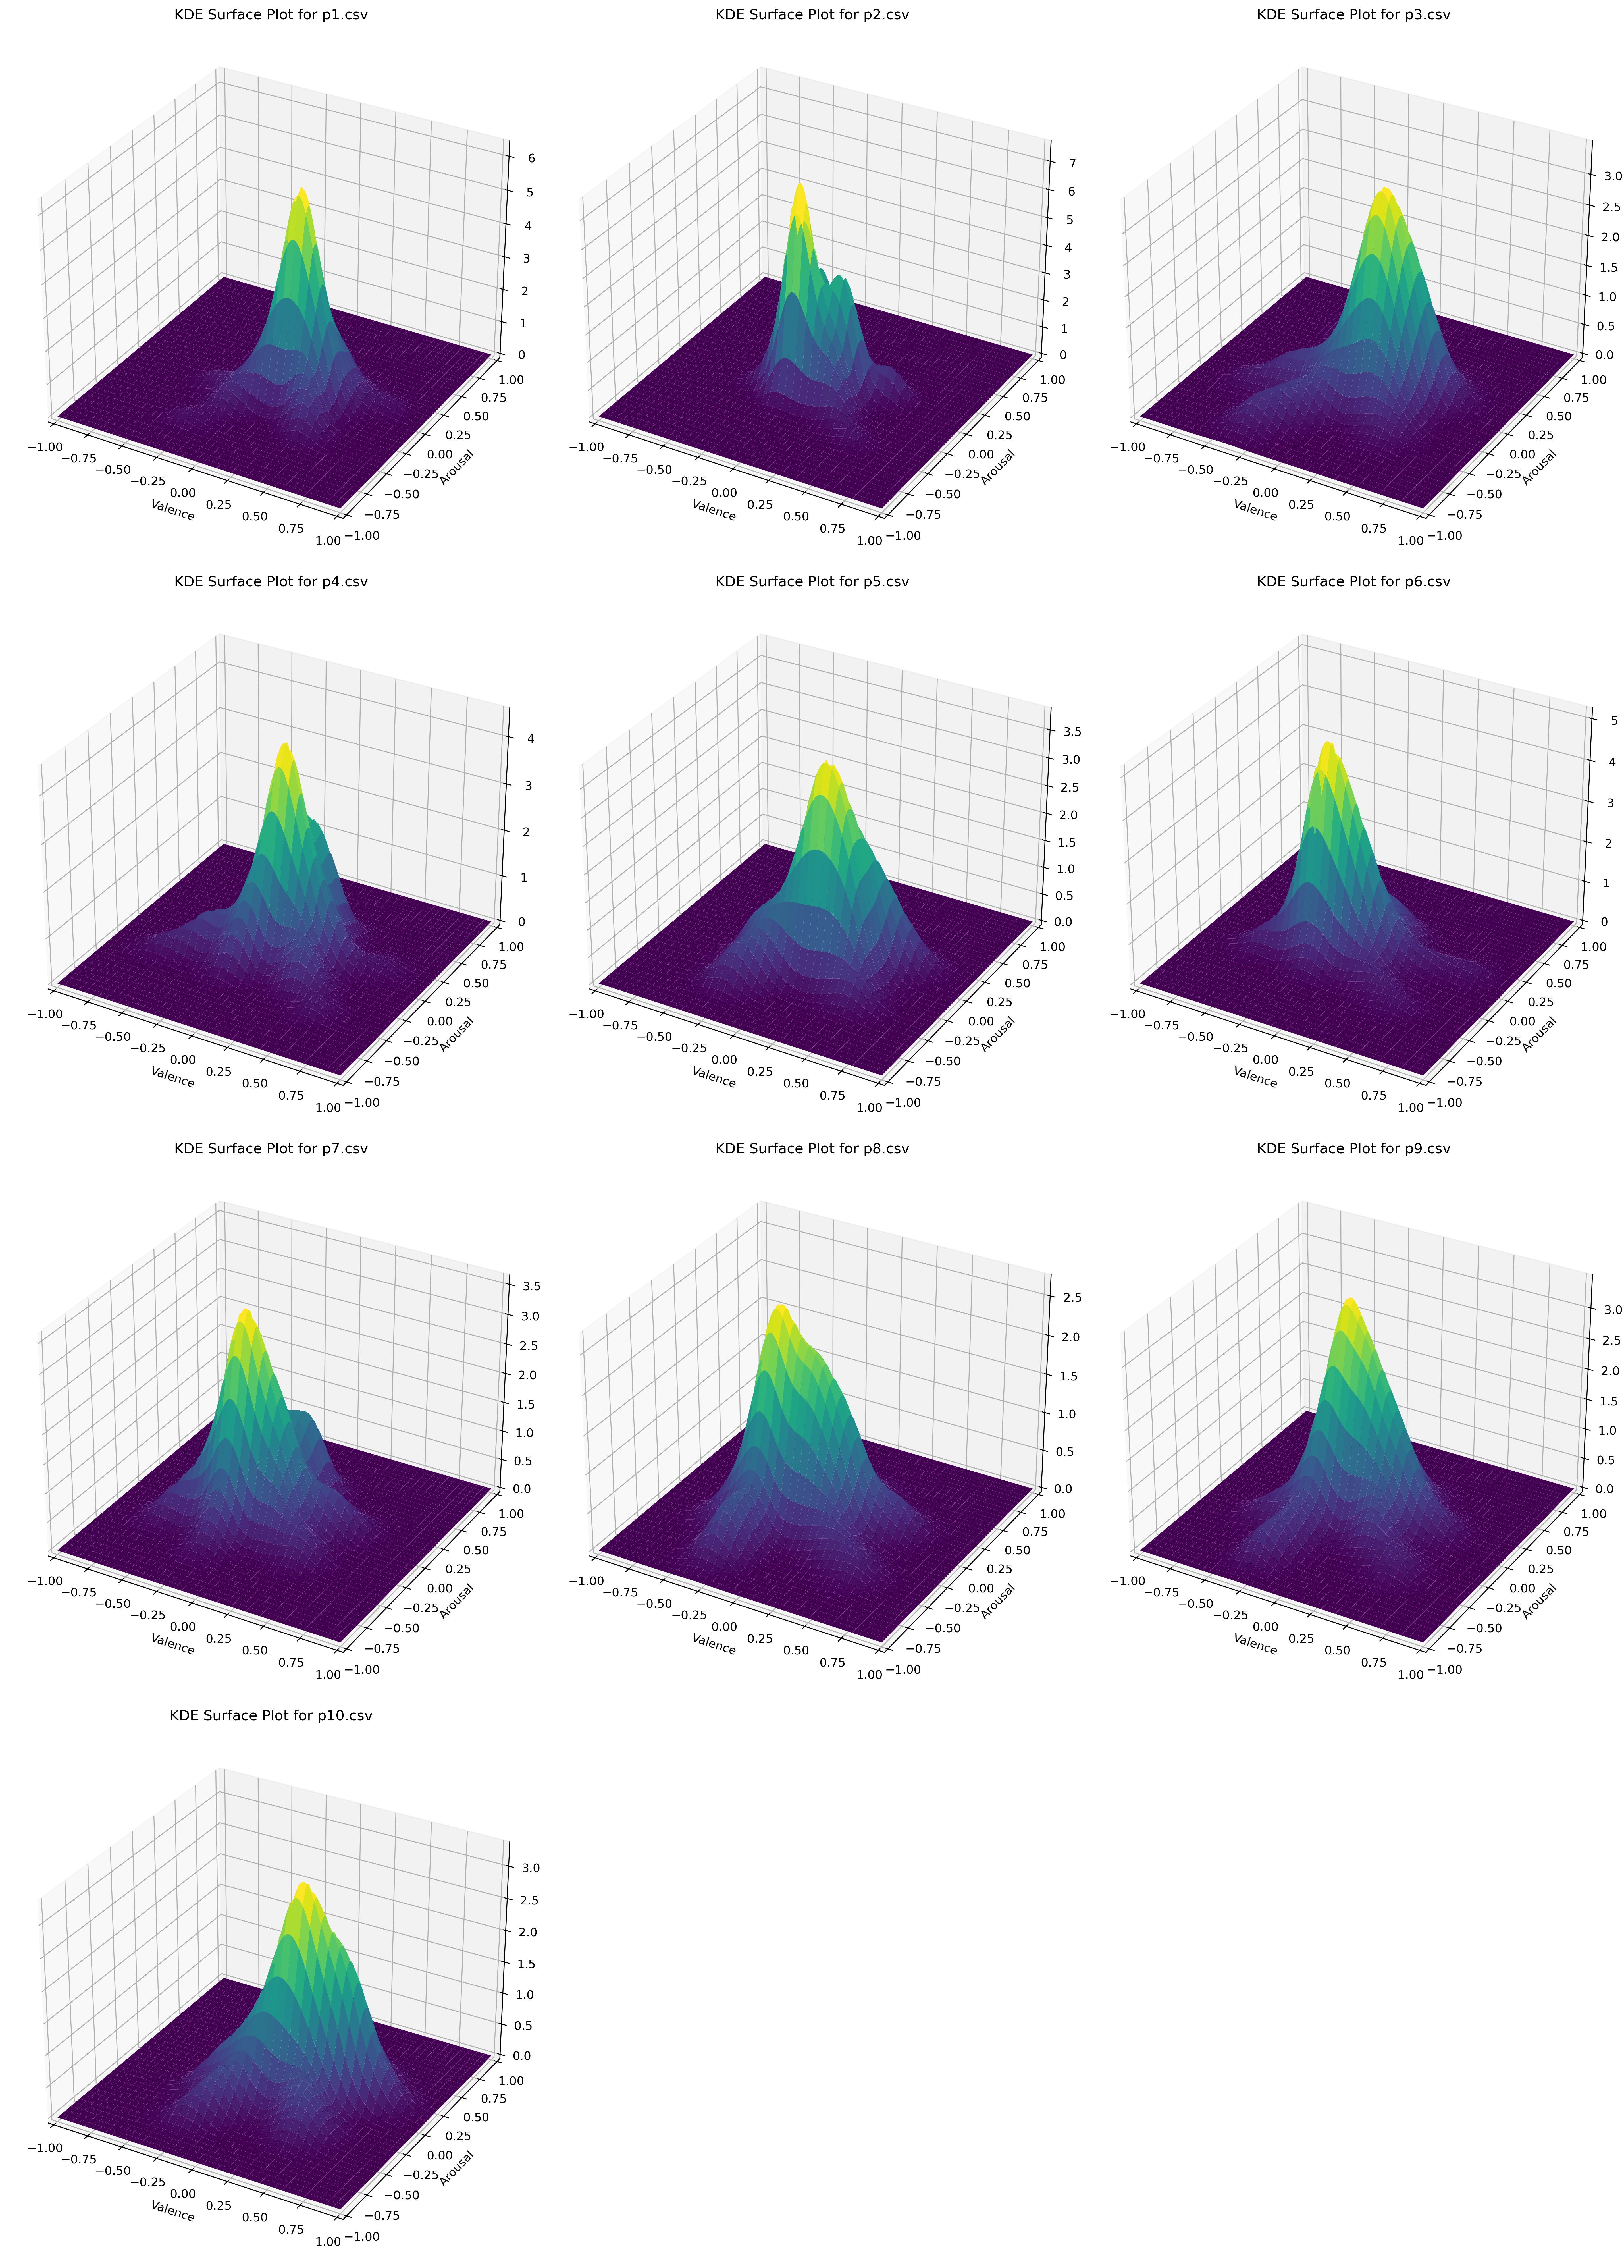
\includegraphics[width=0.80\textwidth]{img/chapter_04/baseline/kde_surface_all-new.png}
    \caption{3D surface plots of KDE-based emotional distributions for all participants}
    \label{fig:kde-3d-plots}
\end{figure}


\begin{figure}[H]
    \centering
    \includegraphics[width=0.80\textwidth]{img/chapter_04/baseline/kde_2d_baseline_map-new.png}
    \caption{2D mapping of KDE-estimated baseline zones for each participant}
    \label{fig:kde-2d-baselines}
\end{figure}


\subsection*{Evaluation}

To evaluate the accuracy and relevance of the identified baseline values, we conducted a questionnaire with all participants. Each participant was asked to reflect on the emotional states represented in their baseline region and indicate how closely those states matched their typical emotional condition during the experiment sessions.

The full questionnaire and participant responses are provided in the Appendix (see Section~\ref{sec:appendix-questionnaire}). Based on the collected responses, we calculated the frequency of agreement between the participants and the computed baseline zones. This frequency distribution is shown in Figure~\ref{fig:baseline-agreement-bar}, which highlights the overall agreement levels across all participants.

In addition, we visualized the relationship between the identified baselines and the participants’ self-reported emotional states using a valence-arousal scatter plot. This comparison, presented in Figure~\ref{fig:baseline-scatter-plot}, helps illustrate how closely the KDE-based baseline aligns with the participants' own perception.

\begin{figure}[H]
    \centering
    \includegraphics[width=0.75\textwidth]{img/chapter_04/baseline/agreement_bar.png}
    \caption{Participant agreement frequency with identified baseline values}
    \label{fig:baseline-agreement-bar}
\end{figure}

\begin{figure}[h]
    \centering
    \includegraphics[width=1\textwidth]{img/chapter_04/baseline/valence_arousal_scatter.png}
    \caption{Scatter plot comparing identified and participant-proposed baseline coordinates}
    \label{fig:baseline-scatter-plot}
\end{figure}


The analysis of the questionnaire responses provides valuable insights into the accuracy and acceptance of the computed baseline values. 

\textbf{General Agreement Level:} The mean agreement score for Question 1  was 3.70 out of 5, indicating that most participants tended to agree with their computed emotional baseline. Furthermore, 60\% of participants explicitly expressed agreement, which supports the reliability of the baseline computation method for the majority.

\textbf{Baseline Discrepancy:} To measure how much the participants’ proposed baselines differed from the computed values, we used the Euclidean distance.
The mean distance was found to be 0.120 with a standard deviation of 0.122. This result shows that, on average, participants' self-identified baseline points differ from the computed values by around 0.12 units in the valence-arousal space. The similarity between the mean and standard deviation also indicates a consistent pattern in how much the computed and proposed baselines deviate from each other. Table~\ref{tab:agreement_summary} summarizes the computed distances for each participant.

\begin{table}[H]
    \centering
    \caption{Participant Agreement and Baseline Discrepancy Summary}
    \begin{tabular}{lcccc}
    \toprule
    \textbf{Participant ID} & \textbf{Agreement (1-5)} & \textbf{Proposed (Valence, Arousal)} & \textbf{Distance} \\
    \midrule
    P1 & 4 & (0.25, -0.05) & 0.054 \\
    P2 & 3 & (0.40, -0.02) & 0.230 \\
    P3 & 4 & (0.20, 0.10) & 0.305 \\
    P4 & 5 & (0.23, -0.06) & 0.014 \\
    P5 & 3 & (-0.05, 0.15) & 0.071 \\
    P6 & 4 & (0.35, -0.10) & 0.054 \\
    P7 & 2 & (0.20, 0.20) & 0.321 \\
    P8 & 4 & (0.24, -0.07) & 0.014 \\
    P9 & 3 & (0.10, -0.05) & 0.134 \\
    P10 & 5 & (0.21, -0.10) & 0.000 \\
    \bottomrule
    \end{tabular}
    \label{tab:agreement_summary}
    \end{table}
    
\section{Phase 4: LLM Response Evaluation}
\label{sec:phase4-llm-evaluation}

In this phase, participants were asked to evaluate the responses generated by the language model based on the procedure outlined in Section~\ref{sec:phase4-llm-responses}. The responses were assessed using a Likert scale across four criteria: \textit{Relevance}, \textit{Emotional Alignment}, \textit{Empathy}, and \textit{Satisfaction}. Each participant rated responses to both a standard (controlled) query and an emotionally-enhanced query.

This evaluation allowed us to compare how the emotional enhancement influenced user perception of the generated responses. The comparison of average ratings between the two types of queries across all four evaluation dimensions is illustrated in Figure~\ref{fig:llm_eval_comparison}.

\begin{figure}[h]
    \centering
    \includegraphics[width=1\textwidth]{img/chapter_04/llm/mean_ratings_comparison.png}
    \caption{Comparison of average ratings for LLM responses}
    \label{fig:llm_eval_comparison}
\end{figure}

\subsection*{Overall Analysis Results}

\begin{table}[H]
    \centering
    \begin{tabular}{|l|c|c|c|c|}
    \hline
    \textbf{Dimension} & \textbf{\makecell{Mean\\Control}} & \textbf{\makecell{Mean\\Enhanced}} & \textbf{\makecell{Mean\\Difference}} & \textbf{\makecell{Improvement\\(\%)}} \\
    \hline
    Satisfaction        & 3.343 & 4.600 & 1.257 & 37.6 \\
    Empathy             & 2.200 & 3.857 & 1.657 & 75.3 \\
    Emotional Alignment & 2.343 & 3.971 & 1.629 & 69.5 \\
    Relevance           & 3.743 & 3.814 & 0.071 & 1.9  \\
    \hline
    \end{tabular}
    \caption{Comparison of participant evaluations for control vs emotionally enhanced responses}
    \label{tab:llm_overall_analysis}
\end{table}


As seen in Table~\ref{tab:llm_overall_analysis}, there is a clear overall increase in user satisfaction, indicating a robust and consistent enhancement in user experience when emotional tailoring is applied. This suggests that emotionally enhanced responses are more engaging and fulfilling for users across various types of queries.

The most significant improvements are observed in \textit{Empathy} (75.3\%) and \textit{Emotional Alignment} (69.5\%), followed by \textit{Satisfaction} (37.6\%). These dimensions, being closely linked to subjective and emotional user experiences, benefit substantially from emotional enhancement. 

On the other hand, the impact on \textit{Relevance} is limited. With only a 1.9\% improvement and a low proportion of participants reporting a positive change as relevance is more dependent on content correctness, which was already adequately addressed by the control responses.

\section{Phase 5: Baseline Refinement}
\label{sec:baseline-refinement}

Following the initial baseline identification, we selected a subset of participants whose self-identified baselines aligned closely with the computed values. This selection was based on their agreement level. The selected participants included P1, P4, P6, P8, and P10. We conducted initial training using those datapoints available around baseline region. 

Subsequently, data was collected during the refinement tasks described in Paragraph~\ref{par:refineing-tasks}.Then observed about the baseline shofts. Initial and refine baseline regions are illustrated in Figure~\ref{fig:baseline-refine-all} for above participants.

\begin{figure}[h]
    \centering
    \includegraphics[width=1\textwidth]{img/chapter_04/b-refine/baseline-refine-all.png}
    \caption{Initial and refined baseline regions for selected participants.}
    \label{fig:baseline-refine-all}
\end{figure}


The results of this section are detailed in Appendix \ref{sec:appendix-refine-questionnaire}, where participant feedback on the refined baselines was collected. As shown in the table, the agreement scores and refined baseline coordinates were evaluated using a Likert scale. Out of the six participants, four (P1, P3, P4, and P6) rated the refined baselines with a score of 4 or higher, indicating agreement with the computed values. This reflects a 66.67\% agreement rate, suggesting that the refined baseline identification method was successful for the majority of users.

\begin{table}[H]
\centering
\caption{Participant Agreement on Refined Baselines}
\begin{tabular}{|c|p{5cm}|c|}
\hline
\textbf{PID} & \textbf{Refined Baseline (V, A)} & \textbf{Likert Score} \\
\hline
P1 & [(0.3, -0.1), (0.4, -0.2)] & 4 \\
P3 & [(0.2, -0.1), (0.3, -0.2)] & 5 \\
P4 & [(0.1, 0.1), (0.2, 0.0)] & 5 \\
P6 & [(-0.2, 0.0), (-0.1, -0.1)] & 4 \\
P8 & [(0.1, 0.2), (0.2, 0.1)] & 2 \\
P10 & [(0.3, -0.1), (0.4, -0.2)] & 3 \\
\hline
\end{tabular}
\end{table}

